\section[General Design Aspects]{General Design Decisions and Aspects of \salespoint{}}
This chapter summarises design decisions and aspects common to all \salespoint{} subsection and details, why those decisions were made.

\subsection{Notes on Interfaces ...\protect\footnote{continued in the next sub-section}}
Integrating a persistence layer into the \salespoint{} Framework had a great impact on some design decisions made during the development of \salespoint{}.
Early on it became obvious that necessities of JPA could dictate the design and implementations of \salespoint{}.

To guard against JPA requirements influencing design decisions, \salespoint{} strongly follows the \textit{programming against interfaces} programming style.
Although, creating an interface for almost every class violates the \textit{KISS} (Keep it simpe, Stupid! Also, a hard-rock band.) principle, the developers deemed programming against interfaces necessary because \salespoint{} is intrinsically tied to JPA.
Using interfaces allowed us to cleanly define the behaviour of an object, without relying on a specific implementation.
The classes itself are, however, not programmed against interfaces.
\salespoint{} usually just implement interfaces, but refer to other classes directly.
The reason for this violation of the \textit{programming against interfaces} paradigm is the generic typing, which would be required, if \salespoint{} classes would refer to interfaces instead of concrete classes.
For example, the \code{PersistentOrder} class would require three (cascaded) generic type parameters alone.
As a consequence, \salespoint{} classes refer to each other directly, instead of interface types.

\subsection{... implementing Classes, and Naming\protect\footnote{started at the preceeding sub-section}}
Objects, which need to be persisted to safe the current state of an application, are called persistence entities.
Usually, a persistence entity is a \textit{Plain Old Java Object} (POJO).
%Separating behaviour and implementation is employed throughout the framework.
However, Java interfaces are used to separate behaviour and implementation.
An interface defines only the behaviour of an object.
Every persistence entity class is an implementation of a corresponding Java interface, to avoid JPA requirements to impact on design decision and, for example, influence the \salespoint{} API.
Each persistence entity has an aggregating class, which also implements an interface.
The interface of an aggregating class specifies its API, but not implementation details.
%Each persistence entity has a manager class, which in turn is an implementation of a manager interface.
%Each persistence entity has an aggregating class, which handles JPA access transparently
Aggregating classes and their respective interfaces are also called manager classes (interfaces), for example \code{UserManager} and \code{OrderManager}.
Sometimes, class and interface names deviate from this naming scheme, for example \code{Calendar}, \code{Inventory} or \code{Accountancy}.
The reason for this break in naming scheme is clarity: because a \code{Calendar} aggregates \code{CalendarEntry}s\footnote{
	The correct plural form would be \code{CalendarEntries}, which is not a type name.
	The form "\code{CalendarEntry}s" is used to support full text search.
	Futhermore, "\code{CalendarEntry}s" should be read as "\code{CalendarEntry} objects" or "objects of the type \code{CalendarEntry}"},
its name according to the scheme would be \code{CalendarEntryManager}.
Everybody knows what a \code{Calendar} is for, but not necessarily what a \code{CalendarEntryManager} does.
Therefore, a more descriptive name was chosen.
The specific manager implementations included \salespoint{} facilitate storing objects to a database.
%However, it is possible to implement every persistence entity and manager class in \salespoint{} non-persistent, for example collection-based.
However, an implementation based on Java collections rather than a database is entirely possible.

\subsection{Why \salespoint{} is so developer-friendly}
\salespoint{} is designed to be developer-friendly.
A crucial part of its easy-to-use feeling is the consistency of interfaces, persistence entities and managers across the framework, including, but not limited to the naming of methods and behaviour of managers.
All aggregating classes share a set of methods, namely \code{add}, \code{get}, \code{contains}, \code{remove} and \code{find}.
The methods have the same semantics on every manager and have a similar method signature.
Concise method names speed up development by reducing typing overhead.
Instead of having an \code{addUser} method for the user manager or an \code{addOrder} method for the order manager, all managers have a method just named \code{add}.
Consistency in the API is achieved by similar method signature.
Consider the \code{get} method: it takes only one parameter which is an identifier.
The precise type of the identifier is easily guessed: the order manager requires an \code{OrderIdentifier} and the \code{Accountancy} an \code{AccountancyEntryIdentifier}.
The name of the identifier type is derived from the name of class which is aggregated by the manager.
This consistency allows a developer to use an unknown manager, when he is familiar with another manager.

\salespoint{} does not contain checked exceptions, thus avoiding ``the handcuffs they put on programmers''~\cite{checked-exceptions}.

%TODO add explanation of iterables
\subsection{Type-based queries in JPA}
\label{jpa-types}
The \code{get()} and \code{find()} methods of aggregating classes in \salespoint{} have a type parameter of \code{Class<E>}.
The type \code{E} is a sub-class of type \code{T}, the generic type parameter of the interface.
For example, the \code{Catalog} interface is generically typed to \code{<T~extends~Product>}, where \code{Product} is an interface itself.
The complete type is thus \code{Catalog<T~extends~Product>}.
\code{PersistentCatalog} implements the generic \code{Catalog} interface with \code{Catalog<PersistentProduct>}.
Thus, \code{PersistentCatalog} aggregates instances of \code{PersistentProduct} or sub-classes thereof.

When \code{Catalog} is queried for \code{Product}s using the \code{get()} and \code{find()} methods, a type parameter has to be supplied.
This type parameter has two purposes: first, it ensures type-safety, and second it narrows the result set.

When a certain type, for example \code{T~extends~PersistentProduct}, is requested from an aggregating class, let's say the \code{PersistentCatalog}, the return type is \code{T} for the \code{get()} method and \code{Iterable<T>}\footnote{More on \code{Iterables} in sub-section~\ref{iterable}.} for the \code{find()} method.
Thus, the return type depends on the request-type and is not a static type, for example \code{PersistentProduct}.
The dependency of the return type on the requested type avoids type casts, which can fail at run-time and therefore increases type-safety.
Because JPA is aware of persistence entities types, the result is always of the correct type, or empty, if no matching object could be found.

The result set determined by the requested type, because the type parameter does not request a specific type, but rather has \code{instanceof} behaviour.
That means, a type parameter does not only match to objects of the same type, but also all objects which have the type of a sub-class of the requested type.
It does not match super-classes of the requested type.
The VideoShop-tutorial\footnote{\url{http://www.st.inf.tu-dresden.de/SalesPoint/v5.0/wiki/index.php/VideoShop}} is an example of how this functionality can be used.
The \code{VideoCatalog} extends \code{PersistentCatalog}.
By using the type parameters \code{Dvd.class} and \code{BluRay.class}, it requires only one line of code to find all products of a certain kind (type).

\begin{figure}
	\centering
  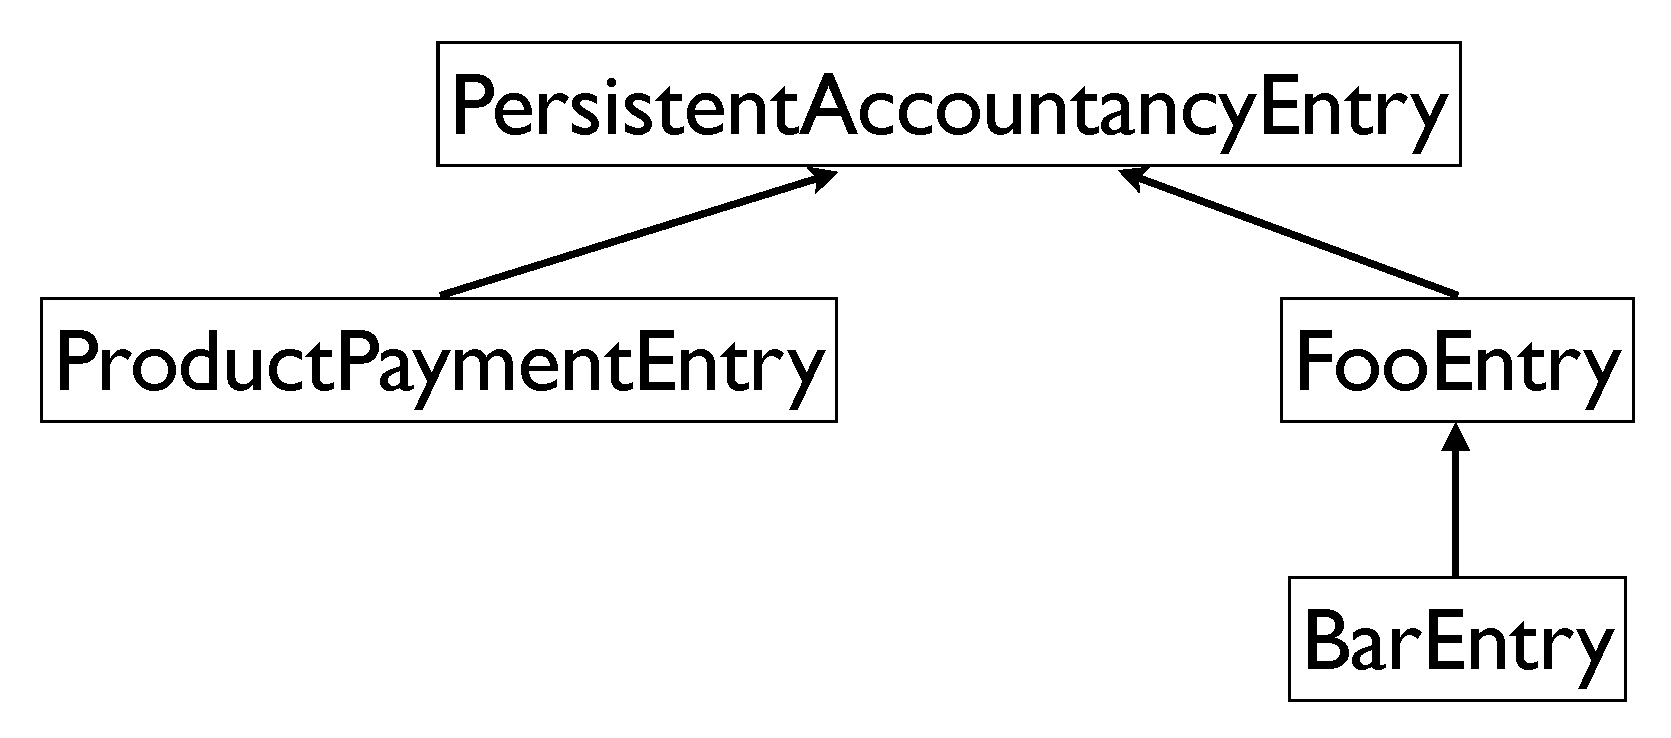
\includegraphics[width=0.5\textwidth]{images/type_matches.pdf}
	\label{matches}
	\caption{Exemplary class hierarchy of \code{PersistentAccountancyEntry}s.}
\end{figure}
\code{PersistenceAccountancyEntry.class} matches all class types.

Consider Figure~\ref{matches} for another example, explaining the \code{instanceof} semantics.
\code{PersistentAccountancy} aggregates \code{PersistentAccountancyEntry}s and sub-classes thereof.
One sub-class is already supplied by \salespoint{}: \code{ProductPaymentEntry}.
\code{ProductPaymentEntry}s are automatically created, if an order is completed.

If \code{ProductPaymentEntry.class} is supplied as type parameter, only objects of type \code{ProductPaymentEntry} would be returned, if any.
Using \code{FooEntry.class} as type parameter would return objects of type \code{FooEntry} and objects of type \code{BarEntry}, if any.
%To access entries of only one type, thus belonging to one ``account'', \code{get()} and \code{find()} methods in \code{Accountancy} have a type parameter.
	

